\documentclass[tikz,border=8pt]{standalone}
% Shared look for every TikZ diagram. Load with % Shared look for every TikZ diagram. Load with % Shared look for every TikZ diagram. Load with \input{../../tools/tikz-style.tex}
\usepackage[T1]{fontenc}
\usepackage{lmodern}
\renewcommand{\sfdefault}{lmr}  % diagrams use the same serif as the text
\usetikzlibrary{arrows.meta, positioning, shapes.geometric, calc, fit, backgrounds}
\definecolor{cblue}{HTML}{4C78A8}
\definecolor{corange}{HTML}{F58518}
\definecolor{cgreen}{HTML}{54A24B}
\definecolor{cred}{HTML}{E45756}
\definecolor{cpurple}{HTML}{B279A2}
\definecolor{cgrey}{HTML}{6B6B6B}
\tikzset{
  every picture/.style={font=\sffamily, line width=1.2pt},
  box/.style={draw=#1, fill=#1!12, rounded corners=4pt, align=center, inner sep=7pt, minimum height=1.1cm},
  box/.default=cgrey,
  arrow/.style={-{Stealth[length=3mm]}, draw=cgrey, line width=1.4pt},
  title/.style={font=\sffamily\bfseries\Large},
  note/.style={font=\sffamily\small, text=cgrey, align=center},
}
\AtBeginDocument{\hyphenpenalty=10000 \exhyphenpenalty=10000}

\usepackage[T1]{fontenc}
\usepackage{lmodern}
\renewcommand{\sfdefault}{lmr}  % diagrams use the same serif as the text
\usetikzlibrary{arrows.meta, positioning, shapes.geometric, calc, fit, backgrounds}
\definecolor{cblue}{HTML}{4C78A8}
\definecolor{corange}{HTML}{F58518}
\definecolor{cgreen}{HTML}{54A24B}
\definecolor{cred}{HTML}{E45756}
\definecolor{cpurple}{HTML}{B279A2}
\definecolor{cgrey}{HTML}{6B6B6B}
\tikzset{
  every picture/.style={font=\sffamily, line width=1.2pt},
  box/.style={draw=#1, fill=#1!12, rounded corners=4pt, align=center, inner sep=7pt, minimum height=1.1cm},
  box/.default=cgrey,
  arrow/.style={-{Stealth[length=3mm]}, draw=cgrey, line width=1.4pt},
  title/.style={font=\sffamily\bfseries\Large},
  note/.style={font=\sffamily\small, text=cgrey, align=center},
}
\AtBeginDocument{\hyphenpenalty=10000 \exhyphenpenalty=10000}

\usepackage[T1]{fontenc}
\usepackage{lmodern}
\renewcommand{\sfdefault}{lmr}  % diagrams use the same serif as the text
\usetikzlibrary{arrows.meta, positioning, shapes.geometric, calc, fit, backgrounds}
\definecolor{cblue}{HTML}{4C78A8}
\definecolor{corange}{HTML}{F58518}
\definecolor{cgreen}{HTML}{54A24B}
\definecolor{cred}{HTML}{E45756}
\definecolor{cpurple}{HTML}{B279A2}
\definecolor{cgrey}{HTML}{6B6B6B}
\tikzset{
  every picture/.style={font=\sffamily, line width=1.2pt},
  box/.style={draw=#1, fill=#1!12, rounded corners=4pt, align=center, inner sep=7pt, minimum height=1.1cm},
  box/.default=cgrey,
  arrow/.style={-{Stealth[length=3mm]}, draw=cgrey, line width=1.4pt},
  title/.style={font=\sffamily\bfseries\Large},
  note/.style={font=\sffamily\small, text=cgrey, align=center},
}
\AtBeginDocument{\hyphenpenalty=10000 \exhyphenpenalty=10000}

\begin{document}
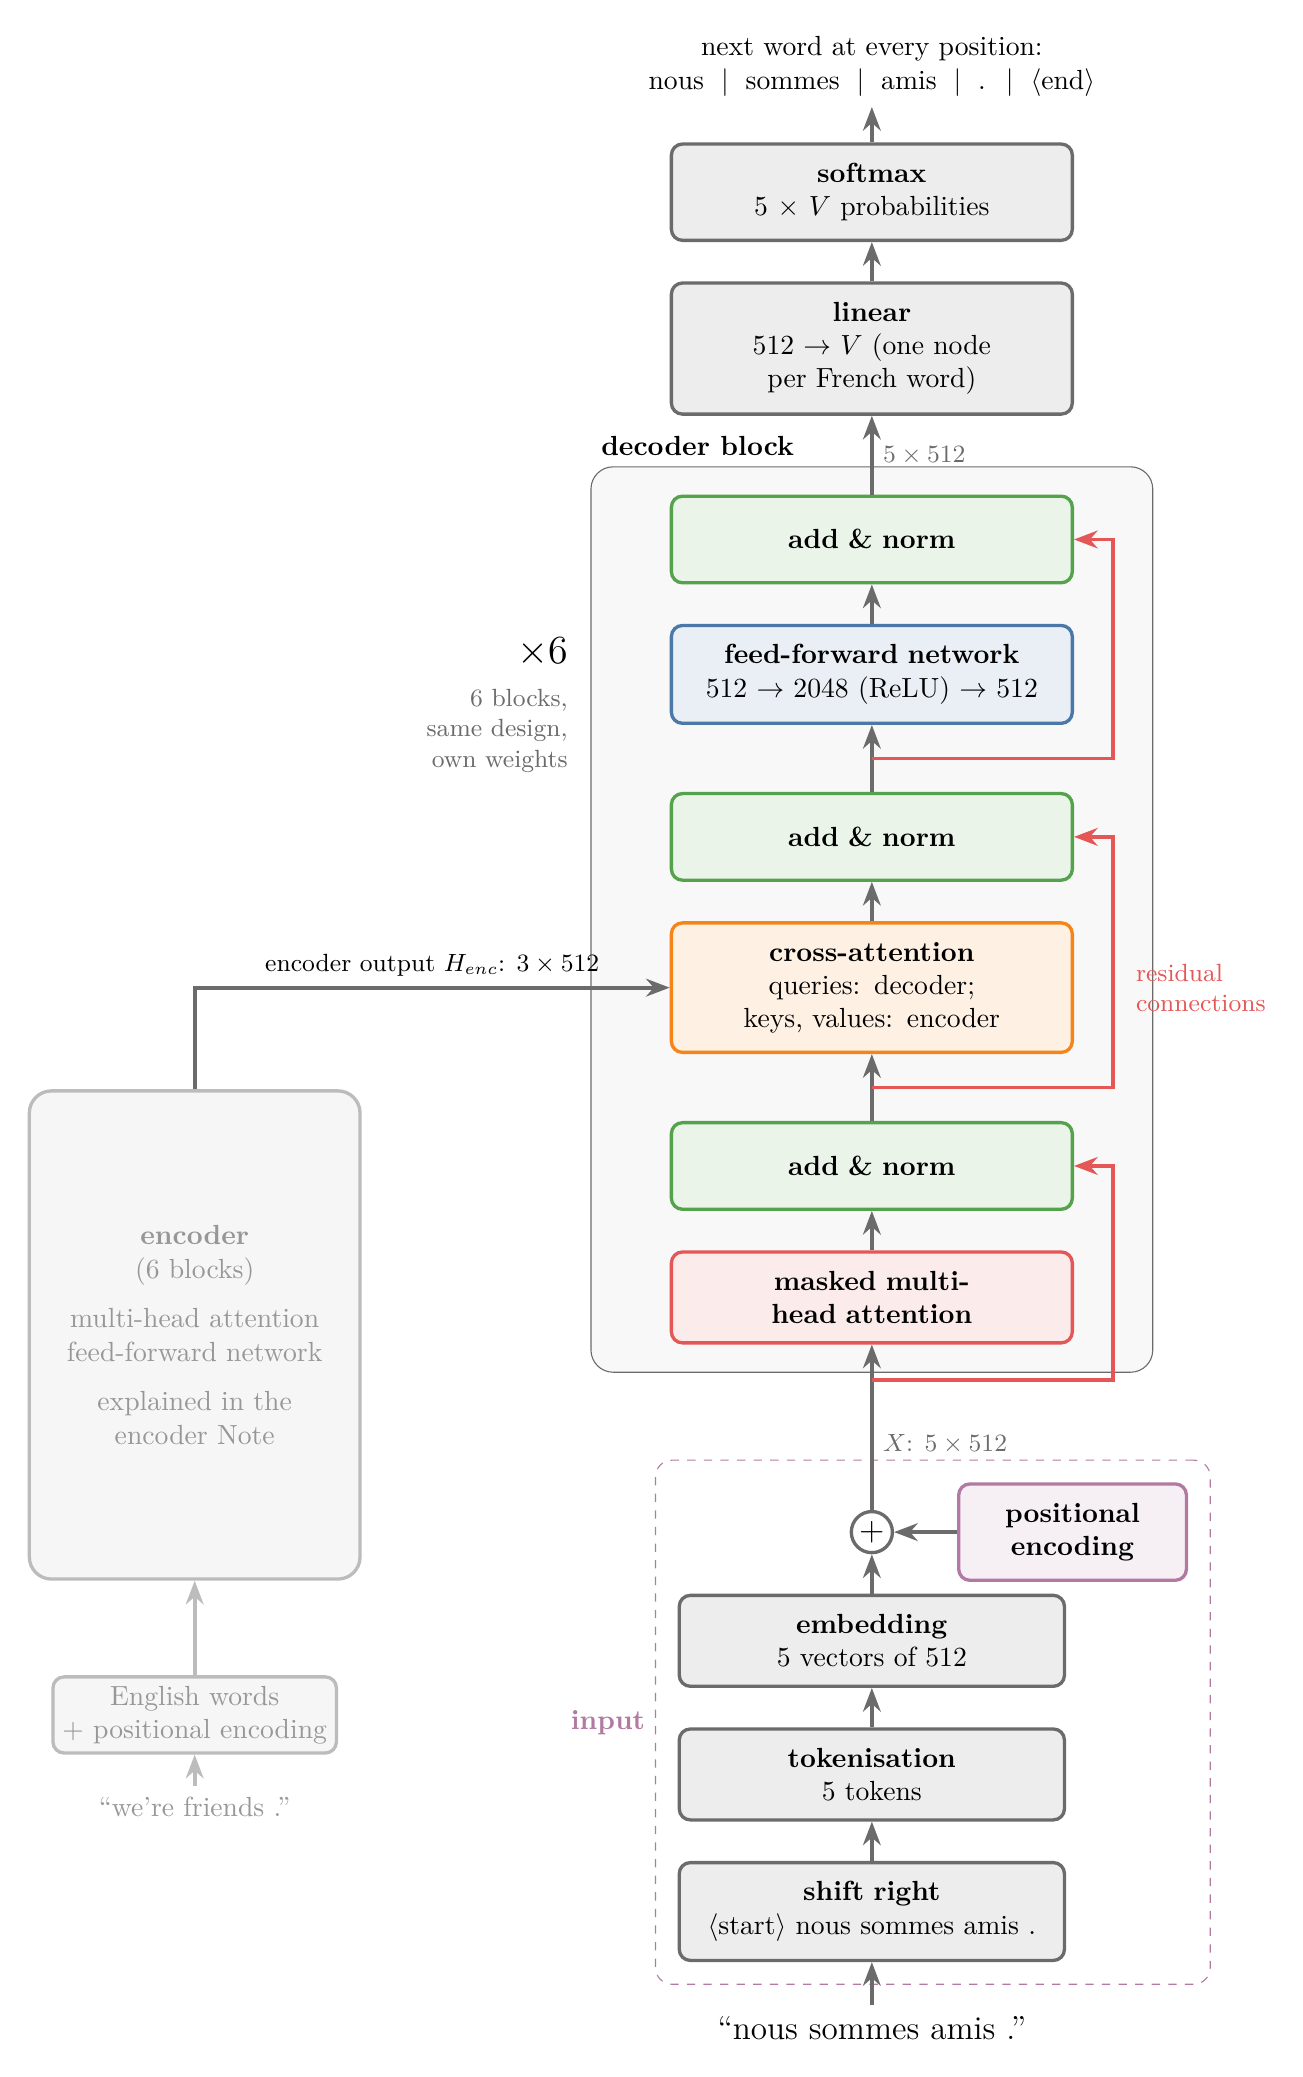
\begin{tikzpicture}[every node/.append style={font=\sffamily}]
  % ---- encoder (greyed, left) ----
  \node[draw=cgrey!45, fill=cgrey!6, rounded corners=8pt, text=cgrey!70, align=center, minimum width=4.2cm, minimum height=6.2cm]
        (enc) at (0,7.6) {\textbf{encoder}\\(6 blocks)\\[6pt]multi-head attention\\feed-forward network\\[6pt]explained in the\\encoder Note};
  \node[draw=cgrey!45, fill=cgrey!6, rounded corners=4pt, text=cgrey!70, align=center, minimum width=3.6cm, below=1.2cm of enc] (ein)
        {English words\\+ positional encoding};
  \node[text=cgrey!70, below=0.4cm of ein] (esent) {``we're friends .''};
  \draw[arrow, draw=cgrey!45] (esent) -- (ein);
  \draw[arrow, draw=cgrey!45] (ein) -- (enc);
  % ---- decoder input (bottom right) ----
  \node[font=\sffamily\large] (sent) at (8.6,-1.2) {``nous sommes amis .''};
  \node[box=cgrey, text width=4.4cm, above=0.55cm of sent] (shift) {\textbf{shift right}\\$\langle$start$\rangle$ nous sommes amis .};
  \node[box=cgrey, text width=4.4cm, above=0.5cm of shift] (tok) {\textbf{tokenisation}\\5 tokens};
  \node[box=cgrey, text width=4.4cm, above=0.5cm of tok] (emb) {\textbf{embedding}\\5 vectors of 512};
  \node[draw=cgrey, circle, inner sep=1pt, font=\large, above=0.5cm of emb] (plus0) {$+$};
  \node[box=cpurple, text width=2.4cm, right=0.8cm of plus0] (pe) {\textbf{positional}\\\textbf{encoding}};
  \draw[arrow] (sent) -- (shift);
  \draw[arrow] (shift) -- (tok);
  \draw[arrow] (tok) -- (emb);
  \draw[arrow] (emb) -- (plus0);
  \draw[arrow] (pe) -- (plus0);
  \begin{scope}[on background layer]
    \node[draw=cpurple, dashed, rounded corners=6pt, fit=(shift)(tok)(emb)(plus0)(pe), inner sep=8pt,
          label={[cpurple, font=\sffamily\bfseries]left:input}] (inbox) {};
  \end{scope}
  % ---- one decoder block ----
  \node[box=cred, text width=4.6cm, above=2.1cm of plus0] (mmha) {\textbf{masked multi-head attention}};
  \node[box=cgreen, text width=4.6cm, above=0.5cm of mmha] (an1) {\textbf{add \& norm}};
  \node[box=corange, text width=4.6cm, above=0.85cm of an1] (cross) {\textbf{cross-attention}\\queries: decoder; keys, values: encoder};
  \node[box=cgreen, text width=4.6cm, above=0.5cm of cross] (an2) {\textbf{add \& norm}};
  \node[box=cblue, text width=4.6cm, above=0.85cm of an2] (ffn) {\textbf{feed-forward network}\\512 $\to$ 2048 (ReLU) $\to$ 512};
  \node[box=cgreen, text width=4.6cm, above=0.5cm of ffn] (an3) {\textbf{add \& norm}};
  \draw[arrow] (plus0) -- node[pos=0.4, right, font=\sffamily\small, text=cgrey] {$X$: $5 \times 512$} (mmha);
  \draw[arrow] (mmha) -- (an1);
  \draw[arrow] (an1) -- (cross);
  \draw[arrow] (cross) -- (an2);
  \draw[arrow] (an2) -- (ffn);
  \draw[arrow] (ffn) -- (an3);
  % residual connections (right side)
  \coordinate (r1) at ([yshift=-0.45cm]mmha.south);
  \draw[arrow, draw=cred] (r1) -| ([xshift=0.5cm]mmha.east) |- (an1.east);
  \coordinate (r2) at ($(an1.north)!0.5!(cross.south)$);
  \draw[arrow, draw=cred] (r2) -| ([xshift=0.5cm]cross.east) |- (an2.east);
  \coordinate (r3) at ($(an2.north)!0.5!(ffn.south)$);
  \draw[arrow, draw=cred] (r3) -| ([xshift=0.5cm]ffn.east) |- (an3.east);
  \node[font=\sffamily\small, text=cred, align=left, right=0.65cm of cross.east] {residual\\connections};
  \begin{scope}[on background layer]
    \node[draw=cgrey, fill=cgrey!5, rounded corners=8pt, fit=(mmha)(an3), inner xsep=1.0cm, inner ysep=10pt] (dec) {};
  \end{scope}
  \node[font=\sffamily\bfseries\Large, anchor=east] at ([xshift=-0.15cm, yshift=3.4cm]dec.west) {$\times 6$};
  \node[font=\sffamily\small, text=cgrey, align=right, anchor=east] at ([xshift=-0.15cm, yshift=2.4cm]dec.west) {6 blocks,\\same design,\\own weights};
  \node[font=\sffamily\bfseries, anchor=south west] at (dec.north west) {decoder block};
  % encoder output into cross-attention
  \draw[arrow] (enc.north) |- node[pos=0.75, above, font=\sffamily\small] {encoder output $H_{\text{enc}}$: $3 \times 512$} (cross.west);
  % output block
  \node[box=cgrey, text width=4.6cm, above=1.0cm of an3] (lin) {\textbf{linear}\\512 $\to$ $V$ (one node per French word)};
  \node[box=cgrey, text width=4.6cm, above=0.5cm of lin] (soft) {\textbf{softmax}\\$5 \times V$ probabilities};
  \node[above=0.45cm of soft, align=center] (outw) {next word at every position:\\nous $\;|\;$ sommes $\;|\;$ amis $\;|\;$ . $\;|\;$ $\langle$end$\rangle$};
  \draw[arrow] (an3) -- node[right, font=\sffamily\small, text=cgrey] {$5 \times 512$} (lin);
  \draw[arrow] (lin) -- (soft);
  \draw[arrow] (soft) -- (outw);
\end{tikzpicture}
\end{document}
